% Options for packages loaded elsewhere
\pdfoutput=1
\PassOptionsToPackage{unicode}{hyperref}
\PassOptionsToPackage{hyphens}{url}
\PassOptionsToPackage{dvipsnames,svgnames,x11names}{xcolor}
\documentclass[
  11pt,
]{article}
\usepackage{xcolor}
\usepackage[margin=1in]{geometry}
\usepackage{amsmath,amssymb}
\setcounter{secnumdepth}{-\maxdimen} % remove section numbering
\usepackage{iftex}
\ifPDFTeX
  \usepackage[T1]{fontenc}
  \usepackage[utf8]{inputenc}
  \usepackage{textcomp} % provide euro and other symbols
\else % if luatex or xetex
  \usepackage{unicode-math} % this also loads fontspec
  \defaultfontfeatures{Scale=MatchLowercase}
  \defaultfontfeatures[\rmfamily]{Ligatures=TeX,Scale=1}
\fi
\usepackage{lmodern}
\ifPDFTeX\else
  % xetex/luatex font selection
\fi
% Use upquote if available, for straight quotes in verbatim environments
\IfFileExists{upquote.sty}{\usepackage{upquote}}{}
\IfFileExists{microtype.sty}{% use microtype if available
  \usepackage[]{microtype}
  \UseMicrotypeSet[protrusion]{basicmath} % disable protrusion for tt fonts
}{}
\makeatletter
\@ifundefined{KOMAClassName}{% if non-KOMA class
  \IfFileExists{parskip.sty}{%
    \usepackage{parskip}
  }{% else
    \setlength{\parindent}{0pt}
    \setlength{\parskip}{6pt plus 2pt minus 1pt}}
}{% if KOMA class
  \KOMAoptions{parskip=half}}
\makeatother
\usepackage{longtable,booktabs,array}
\newcounter{none} % for unnumbered tables
\usepackage{calc} % for calculating minipage widths
% Correct order of tables after \paragraph or \subparagraph
\usepackage{etoolbox}
\makeatletter
\patchcmd\longtable{\par}{\if@noskipsec\mbox{}\fi\par}{}{}
\makeatother
% Allow footnotes in longtable head/foot
\IfFileExists{footnotehyper.sty}{\usepackage{footnotehyper}}{\usepackage{footnote}}
\makesavenoteenv{longtable}
\usepackage{graphicx}
\makeatletter
\newsavebox\pandoc@box
\newcommand*\pandocbounded[1]{% scales image to fit in text height/width
  \sbox\pandoc@box{#1}%
  \Gscale@div\@tempa{\textheight}{\dimexpr\ht\pandoc@box+\dp\pandoc@box\relax}%
  \Gscale@div\@tempb{\linewidth}{\wd\pandoc@box}%
  \ifdim\@tempb\p@<\@tempa\p@\let\@tempa\@tempb\fi% select the smaller of both
  \ifdim\@tempa\p@<\p@\scalebox{\@tempa}{\usebox\pandoc@box}%
  \else\usebox{\pandoc@box}%
  \fi%
}
% Set default figure placement to htbp
\def\fps@figure{htbp}
\makeatother
\setlength{\emergencystretch}{3em} % prevent overfull lines
\providecommand{\tightlist}{%
  \setlength{\itemsep}{0pt}\setlength{\parskip}{0pt}}
\DeclareUnicodeCharacter{2192}{\ensuremath{\rightarrow}}
\DeclareUnicodeCharacter{2190}{\ensuremath{\leftarrow}}
\DeclareUnicodeCharacter{2248}{\ensuremath{\approx}}
\DeclareUnicodeCharacter{03C1}{\ensuremath{\rho}}
\DeclareUnicodeCharacter{03BC}{\ensuremath{\mu}}
\DeclareUnicodeCharacter{2212}{\ensuremath{-}}
\DeclareUnicodeCharacter{2016}{\ensuremath{\|}}
\DeclareUnicodeCharacter{2208}{\ensuremath{\in}}
\DeclareUnicodeCharacter{03B3}{\ensuremath{\gamma}}
\DeclareUnicodeCharacter{03B2}{\ensuremath{\beta}}
\DeclareUnicodeCharacter{00D7}{\ensuremath{\times}}
\DeclareUnicodeCharacter{00B1}{\ensuremath{\pm}}
\DeclareUnicodeCharacter{00B7}{\ensuremath{\cdot}}
\usepackage{bookmark}
\IfFileExists{xurl.sty}{\usepackage{xurl}}{} % add URL line breaks if available
\urlstyle{same}
\hypersetup{
  pdftitle={Train Once{,} Read Everywhere: Substrate Invariance of the Linearly Readable Structure in Frozen Language Models},
  pdfauthor={James Burton Lancaster},
  colorlinks=true,
  linkcolor={blue},
  filecolor={Maroon},
  citecolor={Blue},
  urlcolor={blue},
  pdfcreator={LaTeX via pandoc}}

\title{Train Once, Read Everywhere: Substrate Invariance of the Linearly
Readable Structure in Frozen Language Models}
\author{James Burton Lancaster}
\date{July 25, 2026}

\begin{document}
\maketitle
\begin{abstract}
We report the consolidated findings of the SRT (Semiotic-Reflexive
Transformer) research program: a multi-year effort to treat frozen,
production-scale language models not as black boxes to be fine-tuned but
as \emph{substrates} whose internal states carry structure that small,
inspectable instruments can read. The program's individual results
include a \textasciitilde12M-parameter adapter that exposes per-token
semiotic signals from a frozen 7B backbone with zero cross-entropy
degradation; an activation verbalizer that recovers text from single
hidden states up to a calibrated paraphrase ceiling; read-out ports
spanning architectures from dense 3B to 94-layer 235B-parameter
mixture-of-experts models; and a 22MB linear head that gives a frozen
multimodal chat model image-to-text retrieval at the level of
fully-trained 2018 dual encoders on the standard COCO benchmark.

The headline finding, established in the program's final arc, unifies
these results: \textbf{the readable structure is a stable property of
the model class, invariant along every axis a deployment can vary.} The
cross-modal correspondence inside a frozen multimodal LLM is
anisotropic-linear (a rotation cannot express it; a nonlinear model
finds nothing beyond it at any data scale tested, and falls further
behind as data grows). A head trained once on one host reads, with no
retraining and at most a 42KB recalibration: a host ten times smaller
(31B to 3B, no capability loss at matched data), the same host at 4-bit
weight precision (a 0.011 loss in R@1 with unchanged head weights), and
the same computation on entirely different silicon and kernels
(CUDA/bf16 datacenter to Apple-Silicon/MLX-Q4, 96.7\% head-space
retrieval agreement over the full 5,000-caption pool, read against a
99.6\% same-runtime reproducibility ceiling). Deployment tiers, from
Raspberry-Pi-class edge devices to datacenter fleets, differ in latency
and cost, never in capability. Train once, read everywhere.

We present the instrument stack, the measurement discipline that made
the numbers trustworthy (anisotropy-corrected metrics, anchored
reference frames, controls at every rung), the invariance evidence, and
an honest ledger of the program's negative results, several of which are
load-bearing for the headline claim.
\end{abstract}

\emph{Companion documents: the Stage-3 SRT-Adapter manuscript, the
Stage-4 NLA manuscript, and the engineering guide, all in the program
repository (https://github.com/space-bacon/SRT). Every number in this
paper has a public artifact and a control behind it; the artifact index
is Section 14.}

\subsection{1. Introduction}\label{introduction}

\subsubsection{1.1 The claim}\label{the-claim}

A frozen language model computes more than its output distribution. At
every layer, for every token, it produces intermediate states, and the
SRT program's founding bet was that these states carry \emph{readable}
structure: signals about meaning, divergence, reflexive awareness, and
discourse position that a small instrument can extract without touching
a single backbone weight.

The program's accumulated experiments support the bet, but the result
that organizes all the others arrived last, and it is stronger than the
bet itself. It is not merely that the structure is readable. It is that
\textbf{what the instruments read does not depend on where or how the
substrate runs.} The structure survives a ten-fold change in host scale.
It survives quantization of the weights to four bits. It survives a
change of hardware, numerical kernels, and quantization scheme
simultaneously. And within a multimodal host it is shared across
modalities, connected by a transformation so simple (a single linear map
after per-modality centering) that its entire deployed form fits in 22
megabytes and can be audited by inspection.

We call this property \textbf{substrate invariance}, and we summarize it
operationally: \emph{train once, read everywhere.} An artifact
calibrated against one instance of the model class reads every instance
the deployment world produces, from an edge device performing a single
prefill pass to a datacenter serving a fleet. The tiers differ in
latency and cost. They do not differ in capability.

\subsubsection{1.2 The program in six
stages}\label{the-program-in-six-stages}

\begin{enumerate}
\def\labelenumi{\arabic{enumi}.}
\tightlist
\item
  \textbf{Stages 1--2 (theory and pretraining architecture).} The
  semiotic framework: signs, interpretants, attractor basins of meaning,
  and a proposed architecture with these structures built into the
  embedding layer (Lancaster 2025, SSRN 5987495; Lancaster 2026a, SSRN
  6349978).
\item
  \textbf{Stage 3 (the adapter).} The realization that honest
  instrumentation beats reconstruction: freeze a strong existing model
  and bolt on \textasciitilde12M trainable parameters that read what is
  already latent (\texttt{arxiv/paper.md}).
\item
  \textbf{Stage 4 (activation verbalization).} Reading a single hidden
  state back as text, with the anisotropy-corrected, anchored
  measurement frame that the rest of the program inherited
  (\texttt{paper\_nla.md}).
\item
  \textbf{Stage 5 (scaling the read-out up).} Ports of the read-only
  adapter to gpt-oss-20b and Qwen3-235B-A22B, establishing architecture-
  and scale-generality upward.
\item
  \textbf{Stage 6 (crossing modalities: SRT-Sunstone).} The discovery
  that a text-trained read-out interprets images zero-shot on a frozen
  multimodal host, and the boundary studies that made the claim precise.
\item
  \textbf{The invariance arc (this paper's contribution).} The
  controlled ladder that identified the cross-modal gap as
  anisotropic-linear, benchmarked it, and then deliberately varied
  scale, precision, and hardware to establish that the readable
  structure is invariant.
\end{enumerate}

\subsubsection{1.3 How to read this paper}\label{how-to-read-this-paper}

§2 describes the instruments. §3 describes the measurement discipline;
we consider it a contribution in its own right, because nearly every
number in this field is uninterpretable without it. §4 through §7
present the evidence, organized by invariance axis. §8 assembles the
headline claim. §9 is the ledger of negative results. §10 gives the
semiotic interpretation. §11--§13 situate, scope, and conclude.

\begin{center}\rule{0.5\linewidth}{0.5pt}\end{center}

\subsection{2. The instrument stack}\label{the-instrument-stack}

All instruments share one design rule: \textbf{the backbone is frozen,
byte-identical, and runs natively.} Instruments read hidden states from
forward passes the host is already performing; a deployment gains
capabilities without any risk of regression to the host's primary
function.

\subsubsection{2.1 The SRT-Adapter (Stage
3)}\label{the-srt-adapter-stage-3}

A \textasciitilde12M-parameter module (about 0.17\% of a 7B backbone)
that taps the residual stream of frozen Qwen2.5-7B at three layers.
Metapragmatic Attention Heads (MAH) read divergence; a GRU-based
Reflexive Recurrent Module (RRM) integrates the divergence stream into a
meta-state; a Bifurcation Estimation Network (BEN) emits per-token
reflexivity \(\hat{r}\) and a regime label; a community head discovers
discourse-trajectory structure without labels; and an optional FiLM
correction (\texttt{h\ ←\ h·(1+γ)\ +\ β}) is injected at two layers.
Because the backbone's embeddings and LM head are untouched,
cross-entropy starts at pretrained quality; there is nothing to
``recover.''

Two consumer artifacts ship from this stage: \texttt{srt-adapter-v1.0}
(semantic embeddings; the research series behind it culminated in a
model-soup checkpoint, mean MTEB-STS 0.3744) and \texttt{zooL4nD3r-v0.1}
(961 discourse communities). A separate diagnostic established the
substrate's raw capacity for one downstream task: frozen-backbone
features plus gradient boosting reach TruthfulQA-MC2 AUC 0.8656 ± 0.011
on Qwen2.5-7B (0.8563 on Gemma-2-2B, 0.8475 on Llama-3.2-3B), at the top
of the published hidden-state-detector band (SAPLMA ≈ 0.72; INSIDE ≈
0.78--0.85; EigenScore ≈ 0.80--0.85).

\subsubsection{2.2 The Activation Verbalizer (Stage
4)}\label{the-activation-verbalizer-stage-4}

A \textasciitilde12.7M-parameter head trained so that, given a mid-layer
hidden vector \texttt{v} from the frozen backbone, it generates text
whose own re-encoded activation matches \texttt{v}. Stage 4's lasting
contributions are the measurement frame (§3) and the decoding result:
with oracle best-of-K scoring (legitimate at deploy time, since
\texttt{v} is by construction available), the verbalizer saturates the
paraphrase ceiling at K=64 on Qwen2.5-7B. Its honest limits are equally
important and appear in §9.

\subsubsection{2.3 The linear cross-modal head (the invariance
arc)}\label{the-linear-cross-modal-head-the-invariance-arc}

The simplest instrument in the program and the one that carries the
headline: two linear maps (5376→1024 each, \textasciitilde22MB in bf16)
trained with a symmetric InfoNCE objective on frozen-backbone states of
paired images and captions, plus two per-modality centering vectors
(\textasciitilde42KB). Nothing else. §6 and §7 show what it does and
what it survives.

\begin{center}\rule{0.5\linewidth}{0.5pt}\end{center}

\subsection{3. Measurement discipline}\label{measurement-discipline}

The program's numbers are trustworthy because of four standing rules,
each learned the hard way.

\textbf{Rule 1: always correct for anisotropy.} Transformer hidden
states share a dominant direction; unrelated Qwen2.5-7B L20 states
already have cosine ≈ 0.24 (‖μ‖ ≈ 55), and raw cosine metrics are
therefore uninterpretable. Every similarity in this program is computed
after subtracting the relevant pool mean, and the raw anisotropy is
reported alongside. In the visual channel the same rule reappears with a
refinement (§6.3): the anchor population must be drawn from the query's
own domain, and domain match beats population size.

\textbf{Rule 2: anchor every scale.} Stage 4 metrics are reported as
ρ\_norm ∈ {[}0,1{]}, normalized between a measured random-text floor
(centered fve 0.510 on Qwen L20) and a measured same-source paraphrase
ceiling (0.799), with replay (0.968) and nearest-neighbour retrieval
(0.714) as reference points. A number without an anchored frame is not a
result.

\textbf{Rule 3: every ladder carries controls.} Shuffled-pairs fits
(capacity floors), train-size curves (memorization tests), held-out
splits that are never touched by model selection, and leakage audits.
The Karpathy benchmark run (§6.2) dropped 8,799 training pairs whose
images belong to the Karpathy test and validation splits but had been
moved into train2017 by COCO's 2017 re-partition, and retrained the head
before evaluating.

\textbf{Rule 4: respect encoding conventions.} BOS-sensitivity (a bare
re-encode drops gemma-4 replay from 0.9986 to 0.615), EOS-inclusive
scoring matched between evaluation and calibration, and per-modality
centering are all mandatory and all documented in the released code.

\begin{center}\rule{0.5\linewidth}{0.5pt}\end{center}

\subsection{4. What the taps read on a single
substrate}\label{what-the-taps-read-on-a-single-substrate}

Before invariance can mean anything, the readings themselves must be
established on one substrate. On frozen Qwen2.5-7B the program
established, with full details in the companion manuscripts:

\begin{itemize}
\tightlist
\item
  \textbf{Semantic structure}: the adapter's discourse/embedding vector
  supports competitive semantic similarity (the v1.0 product line and
  its research series).
\item
  \textbf{Reflexivity and regime}: per-token \(\hat{r}\) and a two-class
  regime signal, calibrated well enough that downstream ports report
  expected-calibration errors in the fourth decimal place (§5).
\item
  \textbf{Recoverability of the state itself}: a single L20 hidden state
  is recoverable as text up to the paraphrase ceiling of the backbone
  under best-of-64 oracle decoding (ρ\_cen ≈ 0.99 against the anchored
  frame), with zero-training nearest-neighbour retrieval (ρ ≈ 0.71) as
  the deploy-time fallback that needs no generation at all.
\item
  \textbf{Cross-architecture replication of the substrate claim}: the
  Stage-3 read-off survives 1-NN probes on Qwen3-8B and Mistral-7B-v0.3,
  and the NLA pipeline replicated on Llama-3.2-3B and Gemma-2-2B.
\end{itemize}

\begin{center}\rule{0.5\linewidth}{0.5pt}\end{center}

\subsection{5. Invariance axis one: architecture and scale,
upward}\label{invariance-axis-one-architecture-and-scale-upward}

The read-only adapter ports cleanly to radically different hosts, with
only the \textasciitilde16M side-channel heads trained and the backbone
verified bit-exact against its reference forward pass in each case.

{\def\LTcaptype{none} % do not increment counter
\begin{longtable}[]{@{}
  >{\raggedright\arraybackslash}p{(\linewidth - 8\tabcolsep) * \real{0.1667}}
  >{\raggedright\arraybackslash}p{(\linewidth - 8\tabcolsep) * \real{0.1667}}
  >{\raggedleft\arraybackslash}p{(\linewidth - 8\tabcolsep) * \real{0.2222}}
  >{\raggedleft\arraybackslash}p{(\linewidth - 8\tabcolsep) * \real{0.2222}}
  >{\raggedleft\arraybackslash}p{(\linewidth - 8\tabcolsep) * \real{0.2222}}@{}}
\toprule\noalign{}
\begin{minipage}[b]{\linewidth}\raggedright
host
\end{minipage} & \begin{minipage}[b]{\linewidth}\raggedright
architecture
\end{minipage} & \begin{minipage}[b]{\linewidth}\raggedleft
regime ECE
\end{minipage} & \begin{minipage}[b]{\linewidth}\raggedleft
regime AUROC
\end{minipage} & \begin{minipage}[b]{\linewidth}\raggedleft
community NMI
\end{minipage} \\
\midrule\noalign{}
\endhead
\bottomrule\noalign{}
\endlastfoot
Qwen3-235B-A22B-FP8 & 94-layer MoE, 22B active & 0.0005 & 0.986 &
0.62 \\
gpt-oss-20b (MXFP4) & sliding-window MoE & 0.0009 & 0.974 & 0.42 \\
\end{longtable}
}

The 235B port required sharding across eight GPUs and a
sliding-window-mask implementation verified byte-identical to the
reference; the signals survived unchanged. Reflexivity correlation on
gpt-oss-20b: Pearson 0.689. These ports established upward scale- and
architecture-generality well before the question of \emph{downward}
invariance (§7) was posed.

\begin{center}\rule{0.5\linewidth}{0.5pt}\end{center}

\subsection{6. Invariance axis two:
modality}\label{invariance-axis-two-modality}

\subsubsection{6.1 The zero-shot discovery
(SRT-Sunstone)}\label{the-zero-shot-discovery-srt-sunstone}

A 12.3M community read-out trained on \textbf{text only}, attached to
frozen multimodal gemma-4-31B-it, interprets \textbf{images} with zero
image training: CIFAR-10 image-to-word retrieval@1 of 0.93 against a
chance rate of 0.10, and open-vocabulary retrieval of full sentences
from a pool of ten thousand COCO captions it was never paired with.
Cross-modal alignment peaks at roughly 80\% of backbone depth and
collapses at the final layer, replicating the late-is-surface signature
seen on gpt-oss-20b.

The boundary study made the claim precise. On a random-dot
autostereogram, whose figure exists only in binocular disparity, the
read-out honestly reports texture; a simulated binocular-fusion
front-end recovers the figure from the same pixels, and the read-out
then names it, matching the true-silhouette profile. The capability gap
was in the sensor, not the semiotics. A second boundary, the apparent
inability to retrieve captions for synthetic graphics, was later shown
to be substantially a \emph{calibration artifact}: re-anchoring the
image-side mean on a large natural-photo population moved the
white-heart control's exact caption from rank 352 to rank 5 out of
roughly ten thousand (§6.3).

\subsubsection{6.2 The modality gap is
anisotropic-linear}\label{the-modality-gap-is-anisotropic-linear}

The question the discovery begged: what transformation connects the
image states and the text states? We answered it with a controlled
ladder on COCO pairs (gemma-4-31B-it, layer 47; evaluation split of
1,000 held-out val2017 images against their 5,000 captions, untouched by
any model selection; shuffled-pairs control at every rung).

{\def\LTcaptype{none} % do not increment counter
\begin{longtable}[]{@{}
  >{\raggedright\arraybackslash}p{(\linewidth - 8\tabcolsep) * \real{0.1579}}
  >{\raggedleft\arraybackslash}p{(\linewidth - 8\tabcolsep) * \real{0.2105}}
  >{\raggedleft\arraybackslash}p{(\linewidth - 8\tabcolsep) * \real{0.2105}}
  >{\raggedleft\arraybackslash}p{(\linewidth - 8\tabcolsep) * \real{0.2105}}
  >{\raggedleft\arraybackslash}p{(\linewidth - 8\tabcolsep) * \real{0.2105}}@{}}
\toprule\noalign{}
\begin{minipage}[b]{\linewidth}\raggedright
method
\end{minipage} & \begin{minipage}[b]{\linewidth}\raggedleft
i2t R@1
\end{minipage} & \begin{minipage}[b]{\linewidth}\raggedleft
R@5
\end{minipage} & \begin{minipage}[b]{\linewidth}\raggedleft
R@10
\end{minipage} & \begin{minipage}[b]{\linewidth}\raggedleft
t2i R@1
\end{minipage} \\
\midrule\noalign{}
\endhead
\bottomrule\noalign{}
\endlastfoot
centered cosine (zero training) & 0.288 & 0.523 & 0.648 & 0.173 \\
orthogonal Procrustes (best variant) & 0.247 & 0.506 & 0.656 & 0.164 \\
\textbf{trained linear, 117k pairs, InfoNCE} & \textbf{0.661} &
\textbf{0.911} & \textbf{0.967} & \textbf{0.506} \\
two-layer MLP, 117k pairs & 0.567 & 0.887 & 0.943 & 0.448 \\
shuffled-pairs control & 0.001 & 0.008 & 0.013 & 0.002 \\
\end{longtable}
}

\begin{figure}
\centering
\pandocbounded{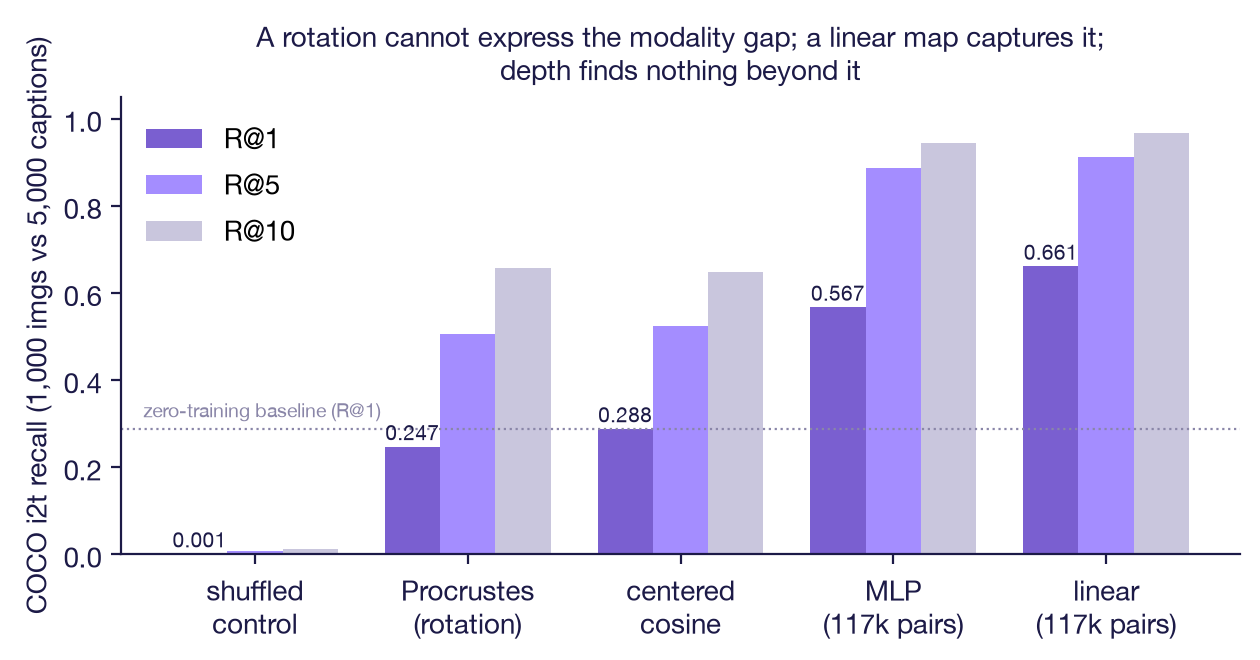
\includegraphics[keepaspectratio,alt={Figure 1. The method ladder. A rotation (orthogonal Procrustes) scores below doing nothing beyond per-modality centering; a single trained linear map captures the gap; a two-layer MLP with the same data never reaches it. Shuffled-pairs control at the floor.}]{figs/fig1_ladder.png}}
\caption{\textbf{Figure 1. The method ladder.} A rotation (orthogonal
Procrustes) scores below doing nothing beyond per-modality centering; a
single trained linear map captures the gap; a two-layer MLP with the
same data never reaches it. Shuffled-pairs control at the floor.}
\end{figure}

Three findings. First, \textbf{a rotation cannot express the gap}: every
orthogonal-Procrustes variant scores below doing nothing beyond
centering, because the two modality means are nearly parallel
(cos(μ\_img, μ\_txt) = 0.979) and the residual difference is a
scale-and-shear that a norm-preserving map cannot fix. Procrustes'
least-squares objective raises absolute paired similarity while
destroying rank discrimination; the objective must optimize ranking.
Second, \textbf{a single linear map captures the gap}, and its ceiling
is still rising at the full COCO supervision (gains decelerate from
roughly +0.10 to +0.06 R@1 per doubling; 0.661 is a lower bound). Third,
\textbf{there is nothing beyond linear to find}: the MLP trails the
linear map at every training size, and the gap \emph{widens} with data
(0.047 at 39k pairs to 0.094 at 117k). Thirty-three times more data
gives the nonlinear model every chance to reveal structure a linear map
cannot express; it instead falls further behind.

\begin{figure}
\centering
\pandocbounded{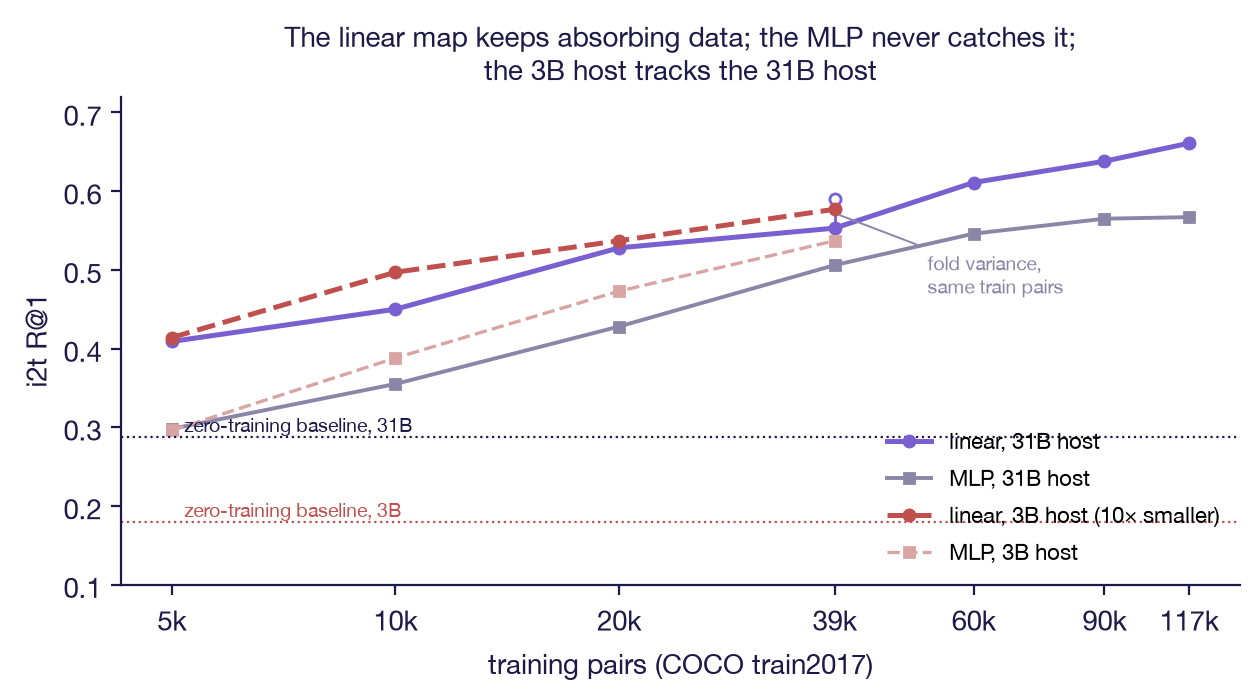
\includegraphics[keepaspectratio,alt={Figure 2. Data scaling and the scale floor in one frame. The linear map absorbs data faster than the MLP at every size on both hosts, and the 3B host's curve tracks the 31B host's: a ten-fold reduction in host scale costs nothing at matched training budget. The two 39k markers on the 31B linear curve show early-stopping fold variance on identical training pairs.}]{figs/fig2_scaling.png}}
\caption{\textbf{Figure 2. Data scaling and the scale floor in one
frame.} The linear map absorbs data faster than the MLP at every size on
both hosts, and the 3B host's curve tracks the 31B host's: a ten-fold
reduction in host scale costs nothing at matched training budget. The
two 39k markers on the 31B linear curve show early-stopping fold
variance on identical training pairs.}
\end{figure}

On the literature-standard \textbf{Karpathy 5k test}, leakage-controlled
as described in §3, the head scores i2t R@1/R@5/R@10 = 0.416 / 0.710 /
0.818 (median rank 2) and t2i 0.292 / 0.567 / 0.685. This matches
fully-trained 2018 dual encoders essentially digit for digit (VSE++:
0.413 / 0.711 / 0.812) from a linear map over a frozen chat model, using
roughly three thousand times less pair data than CLIP-class systems. The
claim is not ``beats CLIP'' (CLIP-class zero-shot sits near 0.58 at
R@1); the claim is \textbf{no new model}: retrieval as a free rider on a
host the deployment already runs.

\begin{figure}
\centering
\pandocbounded{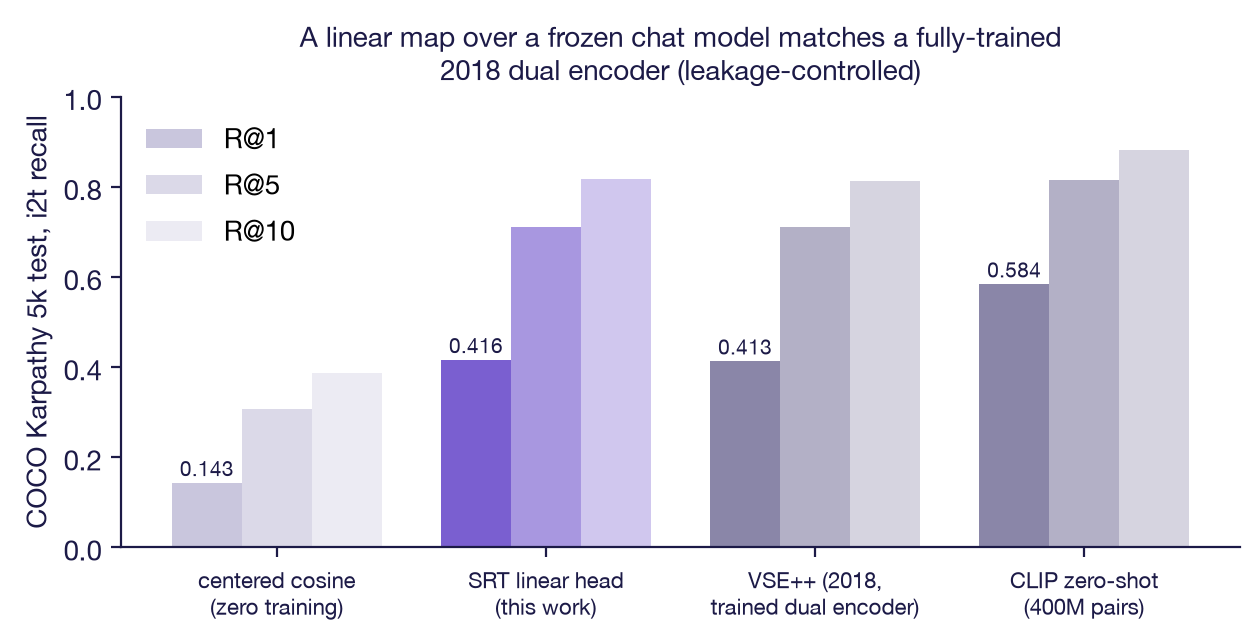
\includegraphics[keepaspectratio,alt={Figure 3. Karpathy 5k placement (leakage-controlled). The linear head over frozen gemma-4-31B-it matches VSE++, a fully-trained 2018 dual encoder, essentially digit for digit, and sits below CLIP-class zero-shot, which trained 400M parameters on 400M pairs.}]{figs/fig4_karpathy.png}}
\caption{\textbf{Figure 3. Karpathy 5k placement (leakage-controlled).}
The linear head over frozen gemma-4-31B-it matches VSE++, a
fully-trained 2018 dual encoder, essentially digit for digit, and sits
below CLIP-class zero-shot, which trained 400M parameters on 400M
pairs.}
\end{figure}

\subsubsection{6.3 The anchor rule,
refined}\label{the-anchor-rule-refined}

The white-heart revision above generalizes Rule 1 to the visual channel
with a twist a control forced on us: re-scoring the demo gallery's
CIFAR-style thumbnails with the 4,000-photo COCO mean \emph{degraded}
their retrievals, while the same mean rescued the synthetic probes
queried against a COCO pool. The anchor population must match the
query's domain, and when domain and size conflict, domain wins: 150
in-domain images beat 4,000 out-of-domain ones. Practically this makes
anchoring a calibration step, not a constant.

\begin{center}\rule{0.5\linewidth}{0.5pt}\end{center}

\subsection{7. Invariance axis three: scale downward, precision, and
hardware}\label{invariance-axis-three-scale-downward-precision-and-hardware}

The final arc varied the three parameters a deployment actually controls
and measured what the head noticed.

\subsubsection{7.1 Host scale: 31B → 3B, no
loss}\label{host-scale-31b-3b-no-loss}

The full ladder was re-run, identical code paths, on frozen
Qwen2.5-VL-3B-Instruct (layer 29 of 36, d = 2048, the same 80\%-depth
heuristic). Every element of the fingerprint reproduced: the
zero-training baseline works (R@1 0.180, 180× chance); Procrustes hurts
(0.147); the trained linear map dominates (0.577 R@1, 0.870 R@5, 0.955
R@10 at 39k pairs, median rank 1); the MLP trails at every size; the
shuffled control sits at 0.000. The decisive comparison is at matched
training budget: the 3B host's 0.577 against the 31B host's 0.553--0.590
(the range reflecting early-stopping fold variance). Within noise,
\textbf{a ten-fold reduction in host size costs nothing.} The linearly
readable cross-modal correspondence is not an emergent luxury of scale;
it is generic to the model class down to at least 3B, and because the
retrieval read-out needs a single prefill pass rather than generation,
3B at 4-bit is Raspberry-Pi-class hardware.

\subsubsection{7.2 Weight precision: bf16 → 4-bit, −0.011
R@1}\label{weight-precision-bf16-4-bit-0.011-r1}

The 3B head, trained on bf16 states, was applied \textbf{unchanged} to
states from the same model loaded in 4-bit NF4:

{\def\LTcaptype{none} % do not increment counter
\begin{longtable}[]{@{}lrrr@{}}
\toprule\noalign{}
configuration & i2t R@1 & R@5 & R@10 \\
\midrule\noalign{}
\endhead
\bottomrule\noalign{}
\endlastfoot
head on bf16 states (reference) & 0.577 & 0.870 & 0.955 \\
same head, unchanged, on 4-bit states & 0.566 & 0.857 & 0.941 \\
plus 42KB mean recalibration & 0.569 & 0.868 & 0.948 \\
\end{longtable}
}

The zero-training baselines are statistically identical across
precisions (0.185 vs 0.180): four-bit quantization barely perturbs the
representation geometry the head reads. A head retrained natively on
quantized states lands on the same data-scaling curve as bf16 training,
confirming that quantized states are fully usable substrate; but the
cross-application result shows retraining is unnecessary. Data budget
matters; precision does not.

\subsubsection{7.3 Hardware and runtime: datacenter CUDA → consumer
Apple
Silicon}\label{hardware-and-runtime-datacenter-cuda-consumer-apple-silicon}

Finally, the original 31B head (trained on CUDA bf16 states in a
datacenter) was tested against states produced by a different
quantization of the same model (MLX 4-bit), running under different
kernels on a consumer machine (Apple M2 Ultra). The protocol is
cross-runtime self-retrieval over the full 5,000-caption calibration
pool, both directions, four arms, with the reference re-encoded fresh on
CUDA to establish a reproducibility ceiling
(\texttt{artifacts/nla/q4/head\_space\_validation\_20260805.json}).

The ceiling first: re-encoding the identical captions on the identical
CUDA runtime reproduces the stored reference at 99.6\% R@1. Bf16 kernel
nondeterminism alone costs 0.4\%, so no cross-runtime number should be
read against 100\%. Across the runtime boundary, raw states retrieve
their datacenter twins at 93.0\% R@1 as-is. Mean-centering alone adds
nothing (93.1\%). \textbf{Through the head}, agreement rises to 96.4\%,
and to \textbf{96.7\% with the 42KB per-runtime mean recalibration}. The
head projects away much of the subspace in which the drift lives: it
learned a stable core of the representation, not its numerically fragile
surface. The drift is not a mean shift; it is structure the head's
5,376-to-1,024 projection discards.

A correction is owed here. An earlier draft of this section reported
98.4\%/100\% and attributed them to head space; a reader's code review
established that the validation script never applied the head (it
measured mean-centered raw states at a smaller pool, where the task
saturates). The numbers above are from the corrected protocol, with the
head applied, and replace the earlier figures. The capability claim for
this tier is scoped to text-side self-retrieval until the image-side
encode is wired on the MLX runtime.

An engineering note with strategic weight: on this consumer runtime the
``state tap,'' the one piece of edge engineering the program had scoped
as remaining work, turned out to require no work at all (the runtime
exposes intermediate states natively). The full stack, a 17GB quantized
31B host plus the 44MB head, runs on a home computer with no GPU server
involved.

\begin{figure}
\centering
\pandocbounded{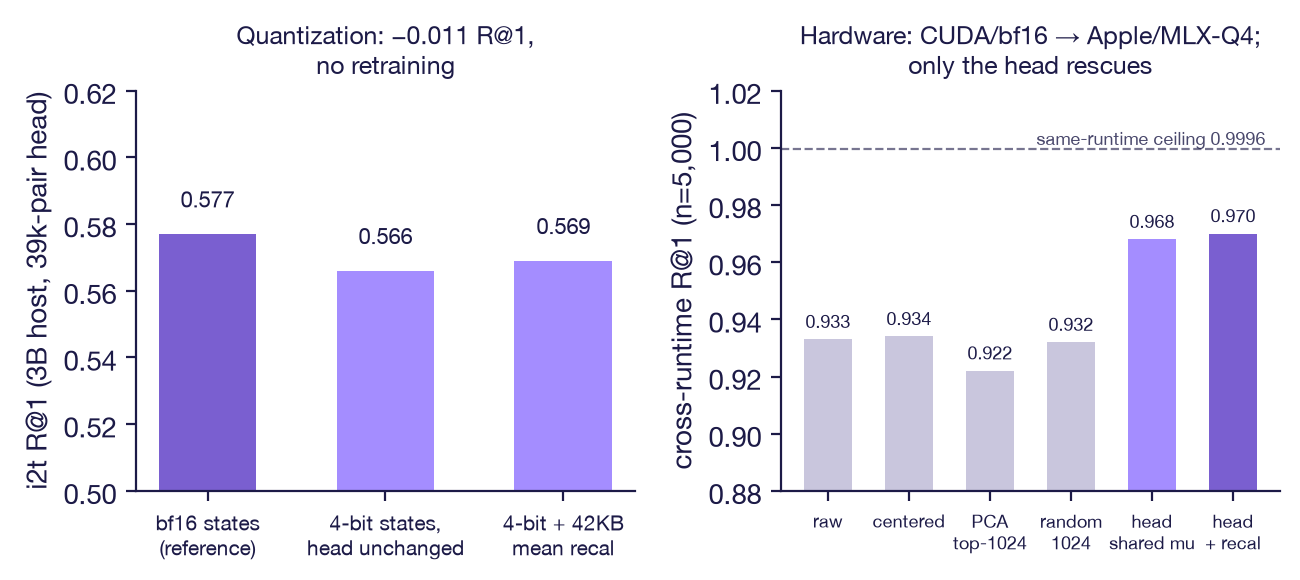
\includegraphics[keepaspectratio,alt={Figure 4. Precision and hardware invariance. Left: the bf16-trained head applied unchanged to 4-bit states loses 0.011 R@1; a 42KB mean recalibration recovers half. Right: across a simultaneous change of hardware, kernels, and quantizer, raw states agree at 93.0\% R@1 over the full 5,000 pool, mean-centering adds nothing, and the head lifts agreement to 96.7\%, against a 99.6\% same-runtime reproducibility ceiling.}]{figs/fig3_invariance.png}}
\caption{\textbf{Figure 4. Precision and hardware invariance.} Left: the
bf16-trained head applied unchanged to 4-bit states loses 0.011 R@1; a
42KB mean recalibration recovers half. Right: across a simultaneous
change of hardware, kernels, and quantizer, raw states agree at 93.0\%
R@1 over the full 5,000 pool, mean-centering adds nothing, and the head
lifts agreement to 96.7\%, against a 99.6\% same-runtime reproducibility
ceiling.}
\end{figure}

\begin{center}\rule{0.5\linewidth}{0.5pt}\end{center}

\subsection{8. The invariance claim,
assembled}\label{the-invariance-claim-assembled}

{\def\LTcaptype{none} % do not increment counter
\begin{longtable}[]{@{}
  >{\raggedright\arraybackslash}p{(\linewidth - 4\tabcolsep) * \real{0.3333}}
  >{\raggedright\arraybackslash}p{(\linewidth - 4\tabcolsep) * \real{0.3333}}
  >{\raggedright\arraybackslash}p{(\linewidth - 4\tabcolsep) * \real{0.3333}}@{}}
\toprule\noalign{}
\begin{minipage}[b]{\linewidth}\raggedright
axis
\end{minipage} & \begin{minipage}[b]{\linewidth}\raggedright
variation
\end{minipage} & \begin{minipage}[b]{\linewidth}\raggedright
result
\end{minipage} \\
\midrule\noalign{}
\endhead
\bottomrule\noalign{}
\endlastfoot
architecture & dense 7B → sliding-window MoE 20B → 94-layer MoE 235B &
read-out signals survive; calibration in the fourth decimal \\
modality & text → images, within one frozen host & shared space; gap is
one linear map \\
host scale (down) & 31B → 3B & identical fingerprint; no loss at matched
data \\
weight precision & bf16 → 4-bit NF4 & −0.011 R@1, head unchanged \\
hardware / runtime / quantizer & CUDA + bnb → Apple Silicon + MLX &
96.7\% head-space agreement (n=5,000) vs a 99.6\% same-runtime ceiling;
head +3.7 over raw, centering inert \\
\end{longtable}
}

The unification: what the SRT instruments read is not a property of a
checkpoint, a precision, a device, or a scale. It is a property of the
\textbf{model class}, stable enough that one small artifact, trained
once, reads it everywhere the class is instantiated. The deployment
consequences follow immediately. A single trained head serves an edge
device batch-tagging photographs overnight, a laptop doing interactive
local search, and a datacenter serving a fleet; every tier runs the
\emph{same artifact} against the \emph{same structure}; and because the
artifact is linear, it can be audited by inspection, and because the
backbone is frozen, the host's primary function carries zero regression
risk. The tiers differ in latency and cost. They do not differ in
capability.

We note the claim's shape: it is an \emph{invariance} claim, and its
strongest evidence is a set of results that would individually be
reported as negatives. Rotation fails. Depth finds nothing. Data does
not rescue the nonlinear model. Quantization does not matter. Scale does
not matter. Each null removes a way the structure could have been
fragile.

\begin{center}\rule{0.5\linewidth}{0.5pt}\end{center}

\subsection{9. The negative-results
ledger}\label{the-negative-results-ledger}

The program treats documented negatives as first-class findings; the
headline could not be trusted without them.

\begin{enumerate}
\def\labelenumi{\arabic{enumi}.}
\tightlist
\item
  \textbf{The greedy gap.} On every host, greedy decoding from the
  activation verbalizer collapses far below retrieval; on
  instruction-tuned hosts the best-of-K curve never reaches the
  retrieval baseline at any practical K (+0.017 per doubling on
  gpt-oss-20b and gemma-4-31B-it, against +0.10 on base Qwen).
  Retrieval, not generation, is the honest decode on tuned hosts.
\item
  \textbf{The base-versus-tuned conjecture, refuted by its own control.}
  An earlier draft conjectured that instruction tuning collapses the
  manifold sampling must traverse. A within-family control (identical
  pipeline on the gemma-4 base checkpoint) produced an indistinguishable
  K-curve (+0.013 vs +0.015 per doubling). Whatever sets verbalizability
  is in the pretrained substrate, not the alignment stage.
\item
  \textbf{Draft-conditioning, refuted with a mechanism.} Conditioning
  the verbalizer on the retrieval neighbour's text adds 0.03 nats of
  predictive value for the gold text; cross-entropy training therefore
  has no gradient toward using it.
\item
  \textbf{Causal injection nulls.} Forcing community prototypes into the
  decode path produces near-zero causal movement on v8a (every diagonal
  effect within ±0.002 nats; the pathway verified live by a
  100×-magnified probe moving CE by +2.27 nats), and the released
  adapters' community-conditioning acts as a uniform style bias rather
  than a per-sign disambiguator. The diagnostic half of the program is
  robust; the causal-steering half is scoped out.
\item
  \textbf{The sensor boundary.} The autostereogram result: no read-out
  can report structure the encoder cannot compute. Supply the missing
  computation (simulated binocular fusion) and the boundary moves.
\item
  \textbf{The anchor artifact.} A published boundary claim (synthetic
  graphics ``outside the domain'') was substantially a calibration
  error, corrected and re-scoped in §6.3. We keep the original claim
  visible in the record because the correction is itself a finding about
  measurement discipline.
\end{enumerate}

\begin{center}\rule{0.5\linewidth}{0.5pt}\end{center}

\subsection{10. Semiotic interpretation}\label{semiotic-interpretation}

The program began in Peircean semiotics, and the invariance result gives
the theory its sharpest empirical footing to date. The
\emph{interpretant}, the effect a sign produces in an interpreting
system, was hypothesized in Stages 1--2 to be a real, structured object
in representational space rather than a theoretical convenience. The
evidence now reads: the interpretant-bearing structure (i) exists in
frozen substrates that were never trained to expose it, (ii) is shared
across the modality in which a sign arrives (word, photograph, or
decoded depth map complete the same interpretant, and name the recovered
figure identically to the real one), (iii) is \emph{linearly} situated,
so that reading it never requires reconstructing the system that
produced it, and (iv) is invariant to the physical realization of the
substrate, which is exactly what one would demand of a structural
property of meaning as opposed to an artifact of a particular network.

The program's law-like battery on contestedness (dissociation, coupling,
causal forcing, and a diachronic test over 11,876 dated articles
spanning 1770--1964, where contested political signs' measured
divergence drifts above concrete controls with a
difference-in-differences of +0.048, permutation p = 0.007, crossing
over in the early twentieth century) locates the semiotic load in the
sign's representation itself rather than in any injectable community
signal, consistent with the causal nulls of §9.4.

\begin{center}\rule{0.5\linewidth}{0.5pt}\end{center}

\subsection{11. Related work}\label{related-work}

The measurement frame descends from the anisotropy literature
(Ethayarajh 2019). The cross-modal ladder engages the cross-lingual
embedding alignment tradition (orthogonal maps between separately
trained spaces) and finds its central tool inapplicable here, for a
reason worth stating: separately trained embedding spaces differ by
rotation-like transforms, but two modalities inside one jointly trained
substrate differ by translation and anisotropic scale. The retrieval
baselines are the standard COCO lineage (Karpathy \& Fei-Fei 2015;
VSE++, Faghri et al.~2018; CLIP, Radford et al.~2021). The hidden-state
diagnostic band is SAPLMA (Azaria \& Mitchell 2023), SAR (Duan et
al.~2024), and INSIDE/EigenScore (Chen et al.~2024). The adapter's
contrastive components use supervised contrastive learning (Khosla et
al.~2020). The theoretical frame is Peirce, read through Kockelman's
semiotic stance and Silverstein's metapragmatics (Lancaster 2025,
2026a).

\subsection{12. Limitations}\label{limitations}

The invariance evidence spans 3B to 235B, three architectures, two
quantization schemes, and two hardware stacks; it does not yet span
model \emph{families} trained by different organizations on the
cross-modal axis (the linear-gap ladder is validated on gemma-4 and
Qwen2.5-VL; the ceiling numbers are gemma-4's). The linear ceiling at
full COCO supervision is a lower bound, not a measured plateau. Sub-3B
hosts are untested. The 4-bit hardware result uses NF4 and MLX-Q4; other
quantizers should track but are unmeasured. Retrieval quality inherits
pool coverage, and anchoring is a genuine calibration step (§6.3) that
deployments must perform. Finally, the causal (injection/steering) half
of the original program remains an open negative: these are reading
instruments.

\subsection{13. Conclusion}\label{conclusion}

The SRT program set out to show that frozen language models are
instrumentable substrates. It ends with something stronger: the
structure the instruments read is invariant across the entire deployment
envelope, scale, precision, and silicon, and cross-modally linear within
a host. The practical corollary is a new class of artifact, small enough
to ship as a configuration file, honest enough to audit by inspection,
that grants a capability wherever its model class runs. The theoretical
corollary is that meaning, as these substrates organize it, is a stable,
linearly readable, realization-independent structure. Train once, read
everywhere.

\begin{center}\rule{0.5\linewidth}{0.5pt}\end{center}

\subsection{14. Artifact index}\label{artifact-index}

\textbf{Models (Hugging Face, \texttt{RiverRider/}):}
\texttt{srt-adapter-v1.0}, \texttt{srt-adapter-v8a},
\texttt{zooL4nD3r-v0.1}, \texttt{srt-adapter-qwen3-235b},
\texttt{srt-adapter-gptoss20b}, \texttt{Gemma-4-31B-it-SRT-Sunstone},
\texttt{srt-sunstone-linear-head} (the 22MB head + anchors),
\texttt{srt-nla-av-v1}, \texttt{srt-nla-av-gemma4},
\texttt{srt-nla-av-llama32-3b}.

\textbf{Data and results
(\texttt{RiverRider/srt-nla-gemma4-artifacts}):} \texttt{procrustes/}
(ladder results, fitted maps, 118k pair encodings, Karpathy eval),
\texttt{scalefloor/} (3B replication + head), \texttt{q4/}
(quantization-drift results + native-Q4 head), \texttt{overnight/} (run
logs and summaries).

\textbf{Code (github.com/space-bacon/SRT):} the adapter and NLA packages
(\texttt{srt/}, \texttt{srt\_introspect/}), the experiment scripts
(\texttt{scripts/gemma4\_procrustes\_xmodal.py},
\texttt{gemma4\_encode\_pairs.py}, \texttt{gemma4\_mlp\_align.py},
\texttt{gemma4\_karpathy\_eval.py}, \texttt{q4\_drift\_eval.py},
\texttt{local\_sunstone.py}), and the engineering guide
(\texttt{docs/CROSSMODAL\_LINEAR\_HEAD.md}).

\textbf{Demos:} \texttt{RiverRider/srt-sunstone},
\texttt{RiverRider/srt-showcase},
\texttt{RiverRider/srt-nla-gptoss20b-trace},
\texttt{srt-adapter-v1.0-demo}.

\subsection{References}\label{references}

\begin{itemize}
\tightlist
\item
  Azaria, A., \& Mitchell, T. (2023). The internal state of an LLM knows
  when it's lying. \emph{Findings of EMNLP}.
\item
  Chen, C., et al.~(2024). INSIDE: LLMs' internal states retain the
  power of hallucination detection. \emph{ICLR}. (Source of the INSIDE
  and EigenScore reference band.)
\item
  Duan, J., et al.~(2024). Shifting attention to relevance: Towards the
  predictive uncertainty quantification of free-form large language
  models. \emph{ACL}. (SAR.)
\item
  Ethayarajh, K. (2019). How contextual are contextualized word
  representations? Comparing the geometry of BERT, ELMo, and GPT-2
  embeddings. \emph{EMNLP-IJCNLP}.
\item
  Faghri, F., Fleet, D. J., Kiros, J. R., \& Fidler, S. (2018). VSE++:
  Improving visual-semantic embeddings with hard negatives. \emph{BMVC}.
\item
  Karpathy, A., \& Fei-Fei, L. (2015). Deep visual-semantic alignments
  for generating image descriptions. \emph{CVPR}.
\item
  Khosla, P., Teterwak, P., Wang, C., Sarna, A., Tian, Y., Isola, P.,
  Maschinot, A., Liu, C., \& Krishnan, D. (2020). Supervised contrastive
  learning. \emph{NeurIPS}.
\item
  Kockelman, P. (2005). The semiotic stance. \emph{Semiotica}, 157(1/4),
  233--304.
\item
  Lancaster, J. B. (2025). The treachery of signs: Semiotic mediation,
  pitchfork bifurcation, and political polarization in algorithmically
  curated societies. SSRN 5987495.
  https://papers.ssrn.com/abstract=5987495
\item
  Lancaster, J. B. (2026a). The Semiotic-Reflexive Transformer: A neural
  architecture for detecting and modulating meaning divergence across
  interpretive communities. SSRN 6349978.
  https://papers.ssrn.com/abstract=6349978
\item
  Lancaster, J. B. (2026b). The SRT-Adapter. Repository manuscript,
  \texttt{arxiv/paper.md}.
\item
  Lancaster, J. B. (2026c). Natural-Language Activations. Repository
  manuscript, \texttt{paper\_nla.md}.
\item
  Peirce, C. S. (1931--1958). \emph{Collected Papers of Charles Sanders
  Peirce} (C. Hartshorne, P. Weiss, \& A. W. Burks, Eds.). Harvard
  University Press.
\item
  Radford, A., Kim, J. W., Hallacy, C., et al.~(2021). Learning
  transferable visual models from natural language supervision.
  \emph{ICML}.
\item
  Silverstein, M. (1976). Shifters, linguistic categories, and cultural
  description. In K. H. Basso \& H. A. Selby (Eds.), \emph{Meaning in
  Anthropology} (pp.~11--55). University of New Mexico Press.
\end{itemize}

\end{document}
